\section{Contexto del sistema y ocho perspectivas}
Pohl presenta ocho perspectivas que ayudan a estudiar el contexto de un sistema sin reducirlo a las pantallas. Para este PFC se utilizan uso, dominio, sistema informático, desarrollo, negocio, innovación, sociedad y técnica. Las preguntas siguientes son una pauta de elicitación para reuniones futuras, y las dos propuestas de cada perspectiva son hipótesis de requisitos, no hallazgos confirmados por ELECTRORIOS \cite{pohl2025,pohlPerspectivas2025}.
\subsection{1. Perspectiva de uso}
\noindent\textbf{Preguntas por contrastar.} ¿Qué pasos sigue el cajero para buscar un artículo?; ¿Quién confirma la venta en horas de alta demanda?; ¿Qué información necesita el comprador para decidir?\par
\noindent\textbf{Propuestas que surgen.} Propuesta: describir por separado búsqueda, cotización y confirmación. Propuesta: conservar un punto de revisión humana antes del cobro.\par
\subsection{2. Perspectiva de dominio}
\noindent\textbf{Preguntas por contrastar.} ¿Cómo se distinguen artículos por voltaje, potencia y fabricante?; ¿Qué unidad de medida se utiliza por producto?; ¿Quién define qué alternativas son técnicamente comparables?\par
\noindent\textbf{Propuestas que surgen.} Propuesta: catalogar atributos eléctricos con unidades consistentes. Propuesta: impedir que una sugerencia sustituya la ficha técnica.\par
\subsection{3. Perspectiva de sistema informático}
\noindent\textbf{Preguntas por contrastar.} ¿Dónde se almacena el stock actualmente?; ¿Cómo se actualizan los precios entre caja y administración?; ¿Qué otros programas están conectados a la venta?\par
\noindent\textbf{Propuestas que surgen.} Propuesta: documentar los intercambios entre venta e inventario. Propuesta: establecer una referencia única para cada operación.\par
\subsection{4. Perspectiva de desarrollo}
\noindent\textbf{Preguntas por contrastar.} ¿Qué personas mantendrán el sistema?; ¿Qué entornos de prueba y despliegue están disponibles?; ¿Cómo se aprobarán cambios al catálogo y a la interfaz?\par
\noindent\textbf{Propuestas que surgen.} Propuesta: versionar los requisitos y sus decisiones. Propuesta: exigir pruebas de regresión antes del despliegue.\par
\subsection{5. Perspectiva de negocio}
\noindent\textbf{Preguntas por contrastar.} ¿Cómo define el local el cierre correcto de una venta?; ¿Qué costos producen los errores de digitación?; ¿Cuáles son las reglas de descuento y devolución?\par
\noindent\textbf{Propuestas que surgen.} Propuesta: documentar las reglas aprobadas de precio y descuentos. Propuesta: registrar diferencias entre cotización y venta final.\par
\subsection{6. Perspectiva de innovación}
\noindent\textbf{Preguntas por contrastar.} ¿En qué situaciones ayudaría una sugerencia de IA?; ¿Cómo evaluará el vendedor su utilidad?; ¿Qué sucede si el servicio no está disponible?\par
\noindent\textbf{Propuestas que surgen.} Propuesta: permitir rechazar una recomendación sin detener la venta. Propuesta: ofrecer búsqueda normal cuando no haya motor de IA.\par
\subsection{7. Perspectiva de sociedad}
\noindent\textbf{Preguntas por contrastar.} ¿Se consideran distintos niveles de experiencia digital?; ¿Cómo se evita exponer datos de clientes?; ¿Qué consecuencias tendría sugerir un material inseguro?\par
\noindent\textbf{Propuestas que surgen.} Propuesta: minimizar datos personales compartidos con servicios externos. Propuesta: mostrar una advertencia de verificación técnica.\par
\subsection{8. Perspectiva de técnica}
\noindent\textbf{Preguntas por contrastar.} ¿Qué ocurre ante dos ventas concurrentes del mismo stock?; ¿Cuánto dura la validez de una respuesta del caché?; ¿Qué campos son obligatorios en cada relación del ER?\par
\noindent\textbf{Propuestas que surgen.} Propuesta: acordar consistencia de inventario y tolerancia a fallos. Propuesta: definir expiración del caché y comportamiento sin conexión.\par

\subsection{Límite del sistema y entidades externas}
La frontera propuesta engloba catálogo, gestión de ventas, roles, registro de consultas y la posible caché local. La relación con otros sistemas necesita estudio: un proveedor, una pasarela o un servicio de IA no se convierten automáticamente en una integración implementada porque aparezcan en el proyecto. La Tabla~\ref{tab:intercambio13} registra cinco interlocutores o servicios con datos, interfaz y frecuencia \emph{propuestos}. En todos los casos se deben confirmar permisos, formatos y disponibilidad \cite{basePFC2026,erPFC2026,pohl2025}.
\begin{table}[!ht]
\centering\scriptsize
\caption{Entidades externas e intercambios preliminares}
\label{tab:intercambio13}
\begin{tabularx}{\columnwidth}{@{}P{1.08cm}Y P{1.02cm}@{}}
\toprule Entidad & Datos previstos y protocolo por definir & Frecuencia posible\\\midrule
Cajero & Búsqueda y venta por interfaz web prevista, aún sin diseño confirmado. & Por atención\\
Cliente & Solicitud de artículo y confirmación de pedido, por interacción humana. & Por compra\\
Proveedor & Catálogo y datos de artículos, mediante archivo o servicio acordado. & Al actualizar\\
Servicio de pago & Estado y referencia de la operación, solo si existe integración contratada. & Por transacción\\
Motor de IA & Códigos y atributos técnicos, sin datos personales; contrato aún pendiente. & Por consulta\\
\bottomrule
\end{tabularx}
\end{table}

\subsection{Lo que aporta el modelo de datos}
El ER que entregó el equipo relaciona ROL con USUARIO; CLIENTE y USUARIO con VENTA; VENTA y PRODUCTO con DETALLE\_VENTA. También asocia PRODUCTO a CATEGORIA y PROVEEDOR. Para las recomendaciones propone CONSULTA\_RECOMENDACION, ligada a USUARIO y opcionalmente a PRODUCTO; para reutilizar respuestas propone CACHE\_TECNICO\_OFFLINE con posibles referencias a CATEGORIA o PRODUCTO \cite{erPFC2026}.

Se trata de un \emph{modelo lógico preliminar}. Antes de tomarlo como base aprobada se necesita decidir si cada registro del caché debe apuntar a una categoría, a un producto o a ambos; cuándo caduca una respuesta; qué sucede cuando se elimina un artículo; y si la asociación de un proveedor a cada producto refleja realmente la compra. Además, el campo \texttt{numero\_factura} no demuestra por sí solo que exista emisión electrónica validada por la administración tributaria.

\begin{figure*}[!t]
\centering
\IfFileExists{figuras/diagrama_er_pfc.png}{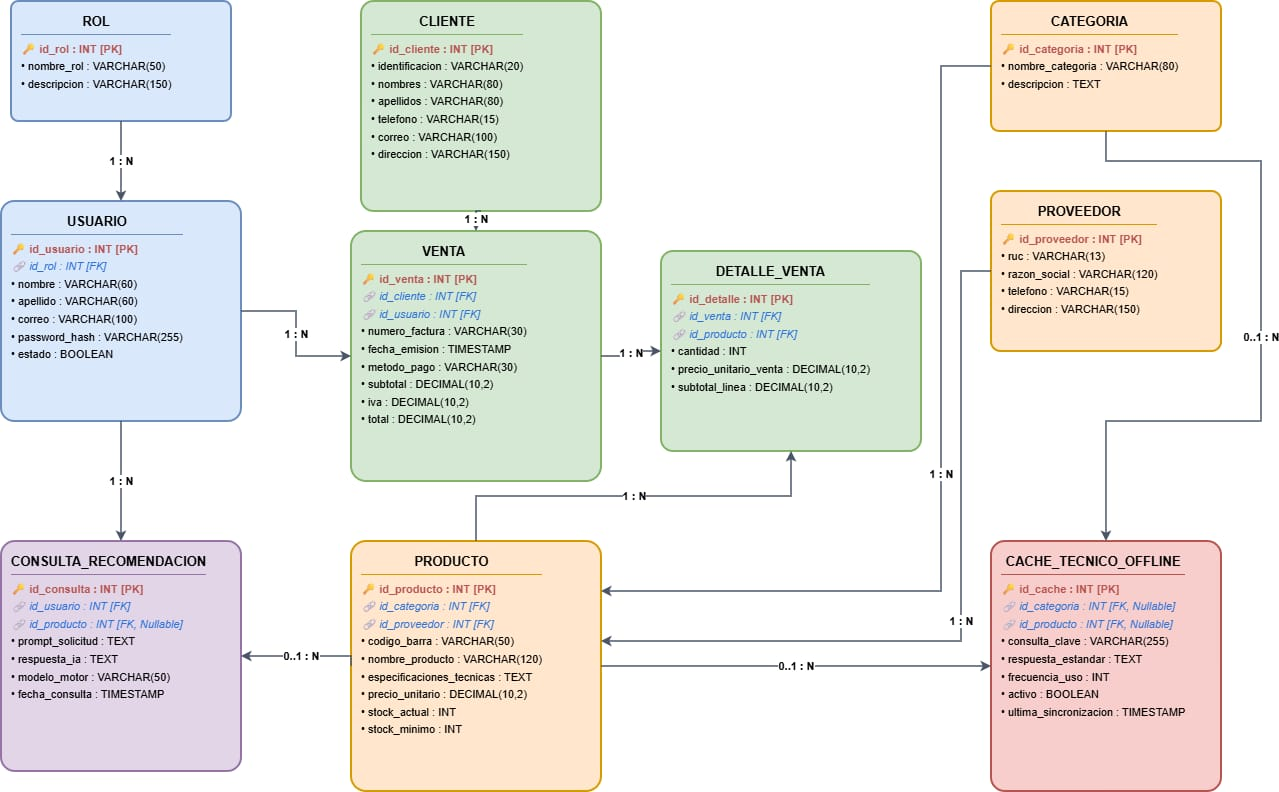
\includegraphics[width=0.91\textwidth]{figuras/diagrama_er_pfc.png}}{\fbox{\parbox{0.82\textwidth}{\centering El diagrama ER está pendiente de subir como imagen. Su versión editable se conserva en la carpeta figuras.}}}
\caption{Modelo entidad-relación preliminar aportado por el equipo, con diez entidades. Se conserva el archivo editable en draw.io. El esquema no representa una base de datos implementada ni validada por el negocio.}
\label{fig:erpfc}
\end{figure*}

\subsection{Preguntas para cerrar el análisis del viernes}
El responsable del almacén deberá confirmar cómo se ajusta el stock después de una venta y una devolución. El personal de caja deberá revisar si la consulta de precios, el orden de las pantallas y la advertencia de recomendación responden a su trabajo habitual. El equipo técnico deberá verificar la viabilidad de la caché y el servicio de IA. Hasta contar con esas respuestas, las métricas y relaciones quedan como propuestas. La Figura~\ref{fig:erpfc} facilita la conversación porque pone en un mismo mapa los datos que podrían verse afectados.

El sábado se propone integrar el mapa conceptual de la unidad, contrastar trazabilidad y preparar la validación del informe con los responsables disponibles, sin presentar como ejecutadas actividades que todavía estén pendientes.
